\documentclass[12pt]{article}

\usepackage[utf8]{inputenc}
\usepackage[francais]{babel}
\usepackage{amsmath}
\usepackage{url}
\usepackage{float}
\usepackage{graphicx}
\usepackage{subfigure}

\title{Recherche de chemin par phéromones} \author{Merwan Achibet $\;$
  \textendash $\;$ Université du Havre} \date{}

\begin{document}

\maketitle

\section*{Introduction}

On se propose d'étudier l'implémentation NetLogo de José M. Vidal
inspirée de \textit{Synthetic Pheromone Mechanisms for Coordination of
  Unmanned Vehicles} de Parunak, Brueckner et Sauter. Dans un premier
temps, on étudie le modèle original puis on analyse l'implémentation
proposée.

\section{Modèle}

\subsection{Analogie avec le vivant}

Les fourmis sont des insectes reconnus pour leur caractère
social. Seules, elles restent vulnérables à l'environnement immense
les entourant. Pourtant, la coopération entre individus de la même
colonie caractérisant cette espèce leur permet de compter parmi les
êtres vivants les plus présents sur le globe terrestre.

Les fourmis communiquent par le biais de signaux chimiques que l'on
peut assimiler à des odeurs, les phéromones \cite{insectes}. Elles
peuvent dialoguer d'individu à individu en utilisant leurs antennes
mais, dans le contexte de la croissance de la fourmilière, il est plus
efficace de déposer dans leur environnement des messages généraux
adressés à tous. C'est notamment le cas lorsqu'une nouvelle source de
nourriture est trouvée puisque la fourmi à l'origine de l'heureuse
découverte déposera derrière elle des phéromones de piste afin que ses
congénères puissent y être guidées. Plusieurs autres types de
phéromones existent : certaines préviennent d'un danger tandis que
d'autre délimitent un territoire ou bien, chez d'autres insectes,
attirent les individus de sexe opposé en période de reproduction.

Les phéromones étant des signaux chimiques éphémères, un phénomène
d'évaporation se produit naturellement et efface progressivement les
pistes.  Pour qu'une piste perdure, elle doit être entretenue par
accumulation des phéromones des autres fourmis l'arpentant. Ainsi
seules les meilleures pistes sont conservées tandis que les autres
(source de nourriture épuisée ou moins importantes) disparaissent par
érosion.  Un aspect important des phéromones est qu'elles sont
soumises à une diffusion dans l'environnement et que les insectes
disposent d'un odorat assez fin pour en retrouver la source. Ainsi, un
individu peut détecter et être attiré par une odeur en passant à
proximité de la piste originelle mais sans nécessairement la croiser.

Ce type de comportement est une source d'inspiration pour la
conception de méthodes de résolution destinée à des systèmes
multi-agents puisqu'il rassemble des qualités notables \cite{parunak}
:

\begin{description}
\item[Diversité]{Une phéromone peut aussi bien indiquer une piste à
  suivre qu'un danger. Le concepteur d'un modèle est libre d'associer
  tout type de sémantique à une phéromone.}
\item[Distribution]{Les signaux chimiques guidant les insectes sont
  répartis sur tout l'environnement.}
\item[Décentralisation]{Si une fourmi est mangée par un oiseau, cela
  n'impactera pas l'avenir de la fourmilière car l'individu manquant
  n'est qu'un rouage d'un mécanisme plus complexe. Les signaux qu'il a
  déposés perdureront jusqu'à évaporation.}
\item[Dynamicité]{Les tracés se renforçant et s'évaporant
  continuellement, les insectes s'adaptent à tout changement impromptu
  de l'environnement.}
\end{description}

Parunak \textit{et al.} partent de ce constat, et s'inspirent des
modèles existants \cite{dorigo}, pour proposer une méthode de guidage
destinée aux véhicules non habités dans le cadre d'opérations
militaires.

\subsection{Les agents et leur monde}

Ici, la fourmi est remplacée par un véhicule, un drone aérien dans
l'exemple. Sa mission est de partir d'une base, et d'atteindre un
bâtiment ennemi cible tout en évitant certaines infrastructures
pouvant l'impacter négativement (radars, batteries anti-aérienne).

Dans la simulation, un véhicule peut déposer deux types de phéromones
:

\begin{description}
\item[GTarget]{Libérée par un agent venant de rencontrer une cible
  ennemi et rentrant à sa base. Elle guide les autres agents vers la
  cible.}
\item[GNest]{Libérée par un agent venant de quitter la base. Elle
  guide les agents vers cette dernière.}
\end{description}

Dans ce modèle, les bâtiments ennemis sont eux aussi agents et
émetteurs des phéromones :

\begin{description}
\item[RTarget]{Libérée par les bâtiments cibles. Elle attire les
  drones.}
\item[RThreat]{Libérée par les bâtiments de contre-mesure. Elle
  repousse les drones.}
\end{description}

Chacune de ces phéromènes véhicule une information différente, mais au
delà de leur sémantique, elles différent aussi de par leur taux de
diffusion dans l'environnement.  Pour les bâtiments ennemis, ce taux
de diffusion dépend de l'aire d'effet du bâtiment associé, et
correspond concrètement à son rayon d'action : le rayon de détection
pour un radar, la portée pour une batterie anti-aérienne.  Le taux de
diffusion des phéromones libérées par les drones doit quant à elle
être finement mesuré pour qu'elles soient remarquées par les véhicules
passant à proximité sans pour autant définir une route trop large (et
donc plus encline à empiéter sur les zones d'effets des bâtiments
ennemis).

L'environnement est divisé en zones (\textit{places}) dont les
dimensions dépendent de la simulation envisagée.  Dans l'exemple SEADy
Storm proposé dans le papier étudié, une zone correspond à une
hexagone de 50 kilomètres de diamètre.  C'est sur ces zones que les
quantités des différentes phéromones déposées sont stockées et aussi
que le phénomène de diffusion se produit entre zones voisines.

Le fonctionnement intrinsèque de ce modèle commence à s'esquisser. Les
phéromones émisent par les différents acteurs de la simulation vont
tisser un canevas de signaux chimiques marquant l'environnement.
Typiquement, les drones auront pour but de suivre une piste menant à
un bâtiment cible tout en évitant les aires d'effet des bâtiments
menaçants, puis à revenir jusqu'à une base.

Les phéromones décrites sont bien sûr spécifiques au modèle présenté
et on peut aisément imaginer, selon la simulation, que l'on en
introduise de nouveaux types. Dans un soucis de généralisme et de
simplicité, on ne souhaite pas qu'un agent ait à envisager des
considérations complexes prenant en compte chaque phéromones
séparement et on préfère associer aux zones une fonction $g$ calculant
leur valeur d'attractivité afin de guider le déplacement des
drones. Dans l'exemple proposé, cette fonction est la suivante, avec
$\alpha$, $\beta$, $\gamma$, $\delta$ et $\theta$ des facteurs de
réglage et $\operatorname{Dist}$ une approximation de la distance
séparant le drone de sa cible :

\begin{equation}
  g = \frac{ \theta \operatorname{RTarget} + \gamma
  \operatorname{GTarget} + \beta}{\alpha \operatorname{RThreat} + \delta
  \operatorname{Dist} + \beta}
  \label{g}
\end{equation}

Lorsqu'un véhicule se trouve dans une zone, il a accès aux quantités
de phéromones présentes dans les zones voisines et un tirage aléatoire
de type roue de la fortune biaisée permet de simuler un choix quant à
la route empruntée.

GHOSTS???

\section{Implémentation}

\subsection{\'Etude}

José M. Vidal a implémenté le modèle décrit précédemment sur la
plate-forme de simulation NetLogo.

Son implémentation est basée sur une grille torique de
\textit{patches} alors que l'implémentation originale utilisait des
hexagones. Cette différence est négligeable au niveau des résultats
que fournit cette simulation car Parunak \textit{et al.} précisent que
la configuration du terrain et des blocs le formant, ainsi que leurs
dimensions peuvent varier librement.

\begin{figure}
  \centering

  \mbox{
    \subfigure{
      \subfigure[RTarget]{
        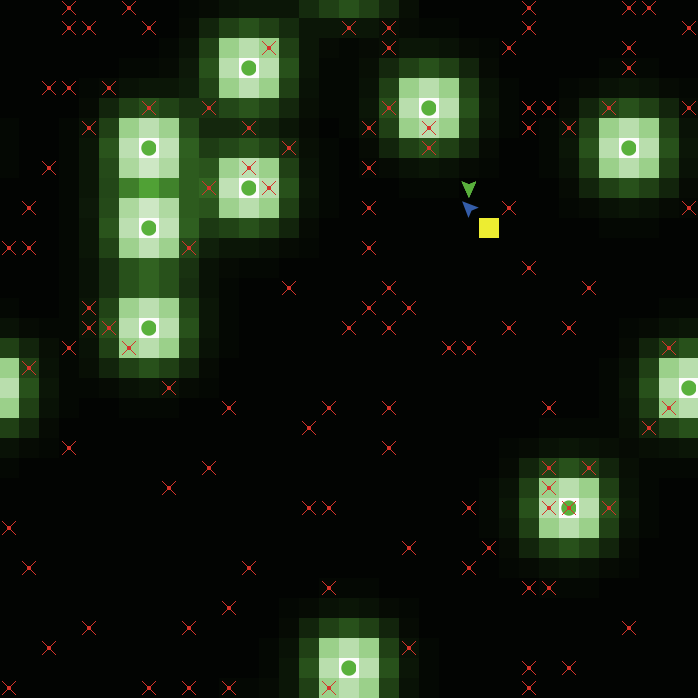
\includegraphics[width=6.5cm]{pheromones_target.png}
      }
      \quad
      \subfigure[RThreat]{
        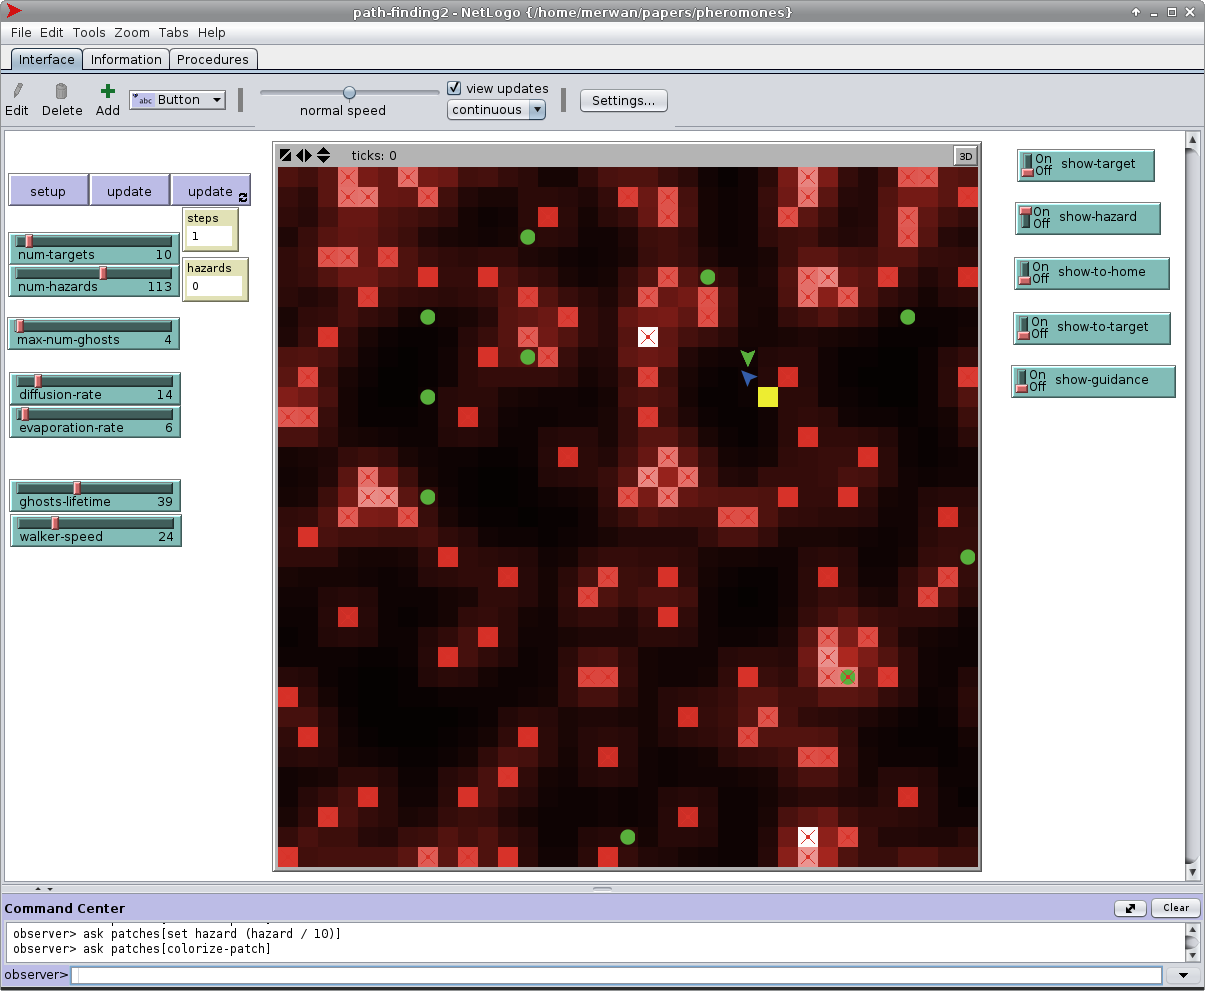
\includegraphics[width=6.5cm]{pheromones_hazard.png}
      }
    }
  }
  \mbox{
    \subfigure{
      \subfigure[GTarget]{
        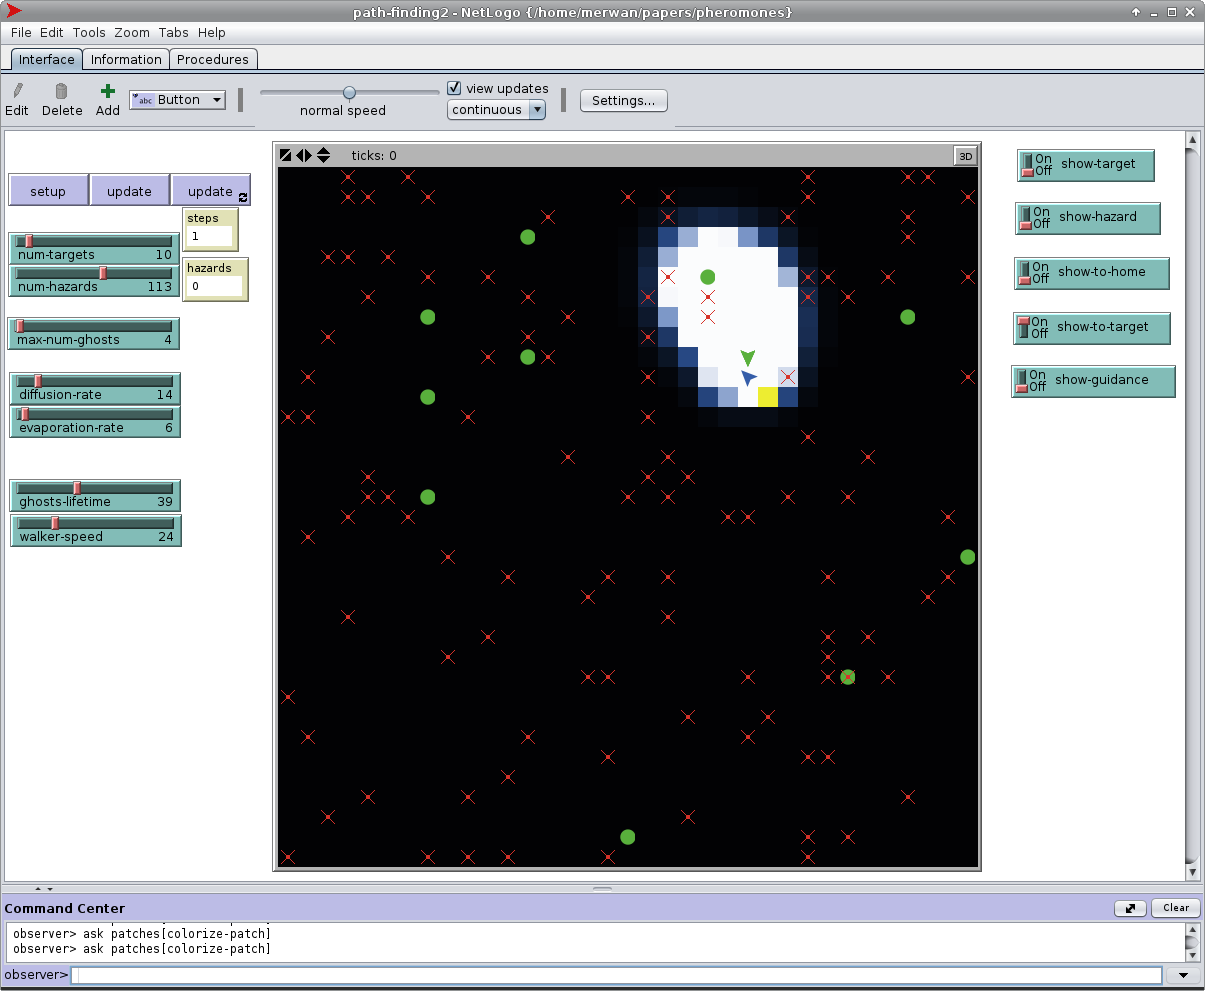
\includegraphics[width=6.5cm]{pheromones_totarget.png}
      }
      \quad
      \subfigure[GNest]{
        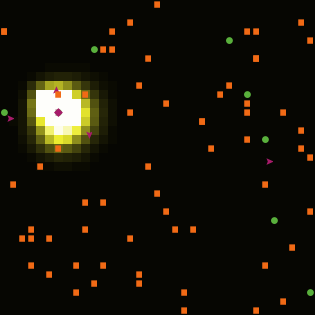
\includegraphics[width=6.5cm]{pheromones_tohome.png}
      }
    }
  }

  \caption{Les quatre types de phéromone pour une configuration donnée}
  \label{pheromones}
\end{figure}

La simulation comprend un unique drone et se termine lorsque ce
dernier atteint une des cibles. Ce drone ayant ici pour unique but
d'atteindre un objectif, il ne fait que se déplacer de \textit{patch}
en \textit{patch} en utilisant comme heuristique la quantité de
phéromone GTarget (menant à une cible) des cases voisines. L'équation
\ref{g} n'est donc pas utilisée. Cette simplification a pour conséquence

EVAP/DIFF

FIN DE LA SIMULATION

FORMULE?

\subsection{Analyse}

Les facteurs que l'utilisateur peut contrôler sont :

\begin{itemize}
\item{Le nombre de cibles}
\item{Le nombre de menaces}
\item{Le nombre maximum de fantômes}
\item{Le taux de diffusion des phéromones}
\item{Le taux d'évaporation des phéromones}
\item{La durée de vie des fantômes}
\item{La vitesse du drone}
\end{itemize}

On remarque que le taux de diffusion ainsi que le taux d'évaporation
est commun à toutes les phéromones, contrairement au modèle original
qui supporte les phéromones disposant de dynamiques différentes.

La durée de vie des fantômes correspond au nombre d'itérations pendant
lequel un fantôme est actif. Lorsque cette limite est atteinte, il
disparaît. Le champ appellé vitesse du drone correspond au nombre
d'itérations

\bibliographystyle{alpha}
\bibliography{sources}

\end{document}
